\documentclass[a4paper,oneside,12pt]{article}

\usepackage[top=3.0cm,bottom=2.0cm,left=3.0cm,right=3.0cm]{geometry}
\usepackage[round,colon,sort]{natbib}
\usepackage[brazil]{babel}
\usepackage{amsmath,amsfonts,amssymb}
\usepackage{graphicx,color}
\usepackage{enumerate}
\usepackage{setspace}
\usepackage[utf8]{inputenc}
\doublespacing % espacamento duplo

\begin{document}

\title{Relatório das Medições dos Sinais de Ângulo de Chegada}
\author{danilopena.ba@gmail.com}
\date{\today}
\maketitle

%----------------------------------------
\section{Introdução}

Relatório para descrição breve e objetiva das aquisições de dados de ângulo de chegada com microfones. Neste relatório será descrito os requisitos, as especificações para aquisição dos dados, restrições e dificuldades. 

%----------------------------------------
\section{Requisitos e Especificações}

As especificações básicas para aquisição de dados em um arranjo de sensores (microfones), garantindo que não haja ambiguidade (\emph{aliasing}) do sinal temporalmente e espacialmente, são:

\begin{itemize}
\item Distância mínima entre os elementos (microfones) do arranjo;
\item Transmissão em campo distante;
\item Frequência de amostragem e largura de banda dos microfones;
\item Largura de \emph{snapshot} (janela) de aquisição.
\end{itemize}

\subsection{Requisitos}

\subsubsection{Distância entre os microfones}

Para evitar a ambiguidade espacial dos dados, equivalente a restrição da frequência de amostragem para estimação espectral, é preciso garantir uma distância mínima entre os microfones, de maneira que os microfones estejam espaçados a uma distância menor que metade do comprimento de onda do sinal.

Se o comprimento do sinal é determinado por:

\begin{equation}
\lambda = \frac{u}{f_c}
\end{equation}

Em que $u$ é a velocidade de propagação do som, e $f_c$ é a frequência máxima da largura de banda do sinal. Como a velocidade da propagação do som é aproximadamente constante (~ $340 m/s$), o comprimento de onda depende da frequência do sinal transmitido. Para as medições iniciais estamos trabalhando com sinais de no máximo $2 kHz$, logo com comprimento de onda de no mínimo $0.17 m$.

O sinal utilizado inicialmente é um tom em $1kHz$, utilizamos uma distância entre os microfones de $0.08 m$ ($8cm$). Posteriormente, para diferentes frequências de tom, e para sinais de voz, será utilizado distâncias menores entre os microfones.

\subsubsection{Transmissão em campo distante}

Para garantir a regularidade do ângulo de incidência entre os sinais nos diferentes microfones, é necessário que o sinal seja transmitido em campo distante. Será utilizado nos experimentos uma restrição de distância mínima entre a fonte e os receptores de dois comprimentos de onda, ou seja, de pelo menos $80 cm$.

\subsubsection{Frequência de amostragem}

Com largura de banda dos microfones de $20kHz$, a aquisição foi especificada para uma frequência de amostragem de $200kHz$, com 10 canais de aquisição.

\subsubsection{Largura de \emph{snapshot}}

A largura do \emph{snapshot} é analisada com valores dentro de uma aquisição de no máximo 400.000 amostras. Cada algoritmo/solução tem sua restrição mínima de tamanho de janela para análise em \emph{short-term}, no caso de algoritmos de análise não-paramétrica o \emph{snapshot} tem largura mínima de 200 amostras (para as especificações de amostragem mencionadas anteriormente), e em soluções de subspaço o \emph{snapshot} mínimo de 10 (número de microfones).

Em análise de \emph{long-term} não é feita avaliação em \emph{snapshots}, e é utilizado todas as 400.000 amostras.

\subsection{Especificações}

O dispositivo de aquisição de sinais utilizado atualmente é o National Instruments NI-6361. Abaixo descrevo as suas características e dos dispositivos utilizados anteriormente a ele.

\subsubsection{ARM TM4C123}

Inicialmente foi utilizado um ARM, da Texas Instruments, Cortex-M4F, no kit LaunchPad (EK-TM4C123GXL), com as seguintes características:

\begin{itemize}
\item CPU 32-bit com frequência de até 80MHz
\item Memórias 256KB Flash, 32KB SRAM, 2KB EEPROM
\item Dois ADCs de 12-bit e 2 MSPS de aquisição
\item Periféricos de comunicação: 8 UART, 6 I2C, 4 SPI
\end{itemize}

Neste microcontrolador foram feitas aquisições de 8 microfones, em 8 canais, como mostrado nas Figuras \ref{fig:arm1} e \ref{fig:arm2}.

\begin{figure}
\centering
\scalebox{0.6}{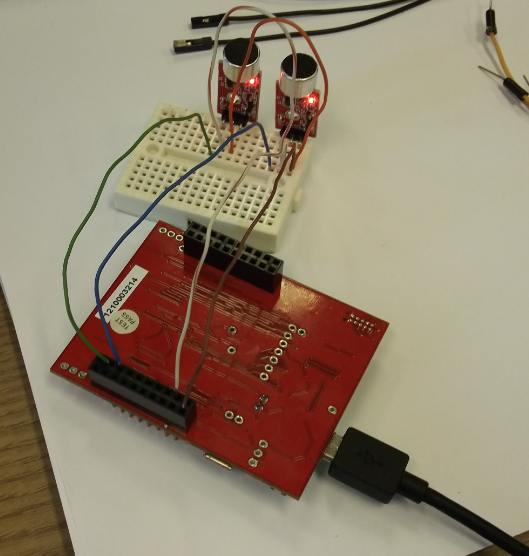
\includegraphics{img1.png}}
\caption{Testes no ARM.}\label{fig:arm1}
\end{figure}

\begin{figure}
\centering
\scalebox{0.6}{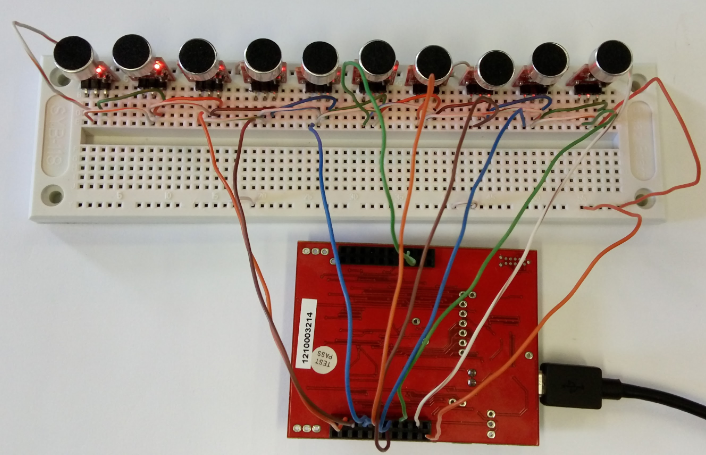
\includegraphics{img2.png}}
\caption{Aquisição no ARM.}\label{fig:arm2}
\end{figure}

\subsubsection{DSP F28027}

Foram realizadas aquisições com o DSP TMS320F28027, da Texas Instruments, com o kit experimental Piccolo LaunchPad (LAUNCHXL-F28027).

O DSP TMS320F28027 tem um processador de 32bits que pode operar até 60MHz (usando PLL), com diversos periféricos, como conversor ADC, módulo PWM, timers de 32bits, oscilador interno (on-chip), PLL, interfaces de comunicação SPI, SCI (UART), I2C, memórias Flash e SARAM.

Possui as seguintes características:

\begin{itemize}
\item Memórias 64KB Flash, 12KB RAM
\item Dois ADCs de 12-bit, 13 canais e 4.6 MSPS de aquisição
\item Periféricos de comunicação: 8 UART, 6 I2C, 4 SPI
\end{itemize}

Neste micro também foram realizadas aquisições com 8 microfones. Dentre as dificuldades, destacam-se a limitação de memória para armazenamento dos dados, o gargalo da largura de banda de transmissão serial para aquisição sem armazenamento de memória, o acesso aos pinos dos canais multiplexados com os demais periféricos.

\subsubsection{Analog Discovery}

Trata-se de um kit aquisitor de dados com entradas diferenciais, como pode ser visto na Figura \ref{fig:analog}, com aquisição de até 100 MSPS, profundidade de 14-bit, com até 16 Ksa/canal, e largura de banda de 5 MHz. O número total de canais são 16, ou 8 diferenciais.

Neste aquisitor utilizou-se o \emph{software} Waveforms para gravação da aquisição e exportação dos dados, que em seguida eram passados para análise no Matlab. A dificuldade ficou por conta da dependência do \emph{software}, apesar de já existir suporte atual de \emph{Hardware} para o Matlab.

\begin{figure}
\centering
\scalebox{0.6}{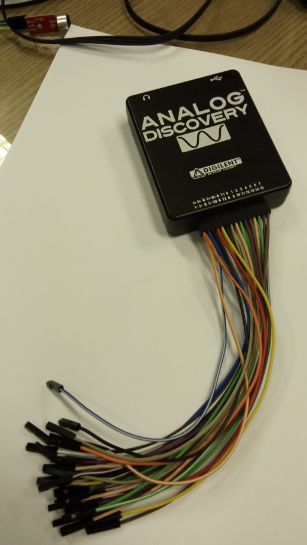
\includegraphics{img3.png}}
\caption{Analog Discovery.}\label{fig:analog}
\end{figure}

\subsubsection{National Instruments NI-6361}

Por fim, foi utilizado o aquisitor NI-6361 da National Instruments, que utilizo até hoje, como mostrado na Figura \ref{fig:NI}. Ele possui 16 canais sendo 8 diferenciais. Com taxa de aquisição de 2 MSPs, e máximo de 1  MSPs por canal, com saídas analógicas e digitais, que são úteis para alimentação dos microfones. O \emph{software} utilizado é o SignalExpress da NI, onde é registrado o log das aquisições e exportado em arquivos .tdms, que em seguida é convertido para .mat no Matlab.

\begin{figure}
\centering
\scalebox{0.4}{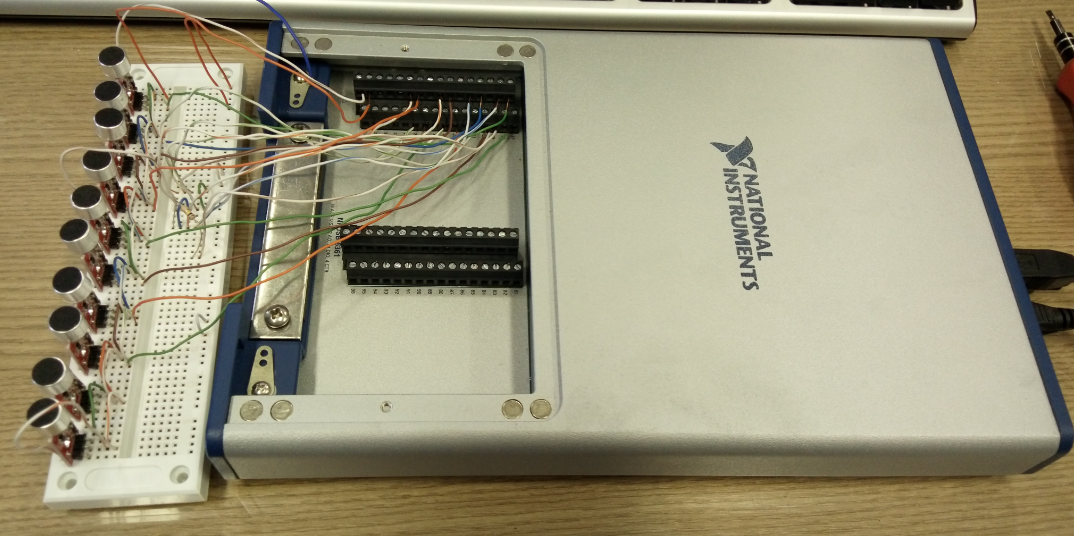
\includegraphics{img4.png}}
\caption{NI-6361.}\label{fig:NI}
\end{figure}

Foram testados medições diferenciais e os resultados quanto a ruído/interferência foram melhores, porém as medições foram realizadas com terra comum, não sendo diferencial, pois não há canais suficientes.

%----------------------------------------
\section{Aquisições}

Sob orientação do Prof. Vicente, e com ajuda de dois alunos de seu laboratório, Carlos e Matheus, desenvolvemos uma mesa para suporte, conforme Figura \ref{fig:mesa}. A mesa conta com rodinhas para auxiliar a mobilidade, além de ser leve. O objetivo é que seja de fácil locomoção para que se possa fazer aquisições em diversos ambientes.

\begin{figure}
\centering
\scalebox{0.6}{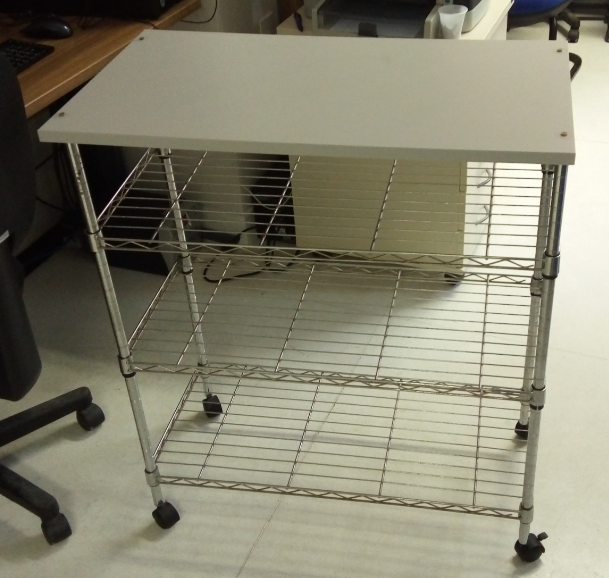
\includegraphics{img5.png}}
\caption{Mesa de suporte.}\label{fig:mesa}
\end{figure}

Em cima da mesa colocamos os microfones uniformemente espaçados, e o aquisitor NI-6361, como mostrado na Figura \ref{fig:mesa_microfone}.

\begin{figure}
\centering
\scalebox{0.4}{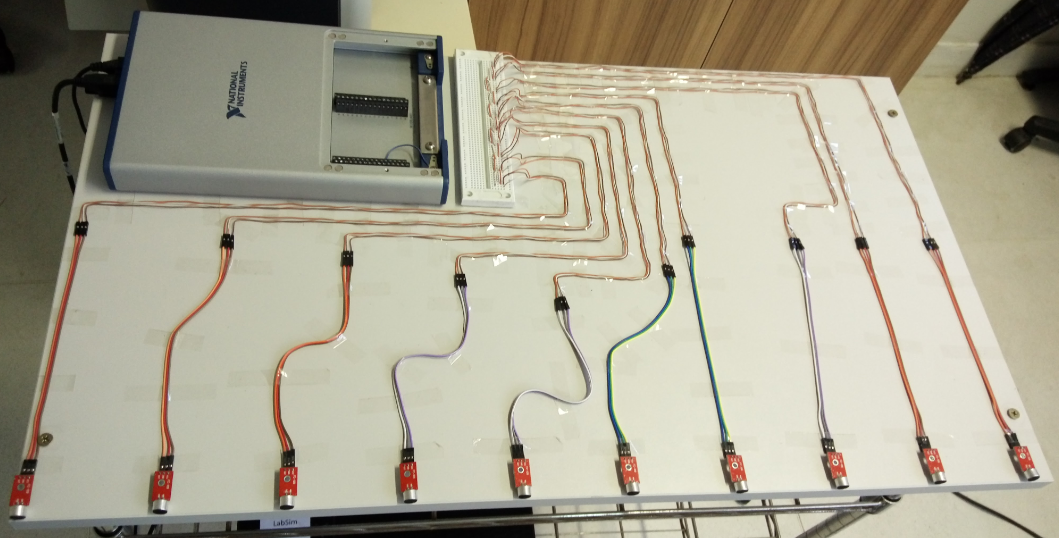
\includegraphics{img6.png}}
\caption{Microfones e aquisitor na mesa.}\label{fig:mesa_microfone}
\end{figure}

Na parte de baixo da mesa, existem prateleiras, que é possível dar suporte ao notebook que realiza o log dos dados. Como mostra na Figura \ref{fig:mesa_notebook}.

\begin{figure}
\centering
\scalebox{0.6}{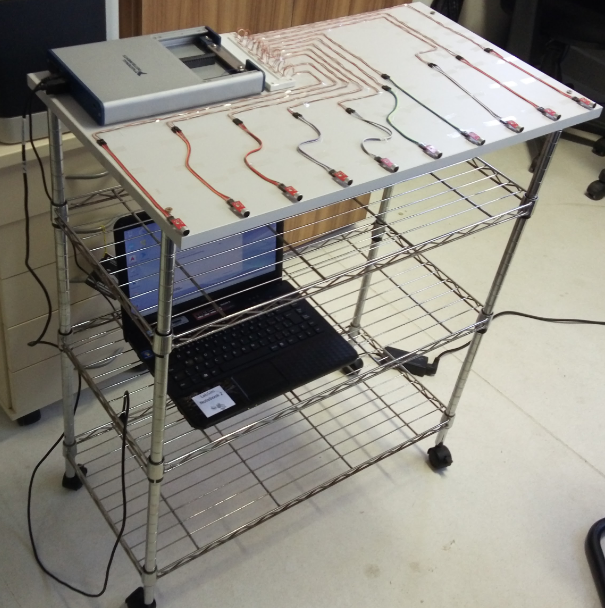
\includegraphics{img7.png}}
\caption{Notebook na mesa.}\label{fig:mesa_notebook}
\end{figure}

As principais baterias de aquisições foram realizadas no salão principal do prédio do CTEC, como mostra a mesa montada para aquisição na Figura \ref{fig:mesa_pronta}.

\begin{figure}
\centering
\scalebox{0.6}{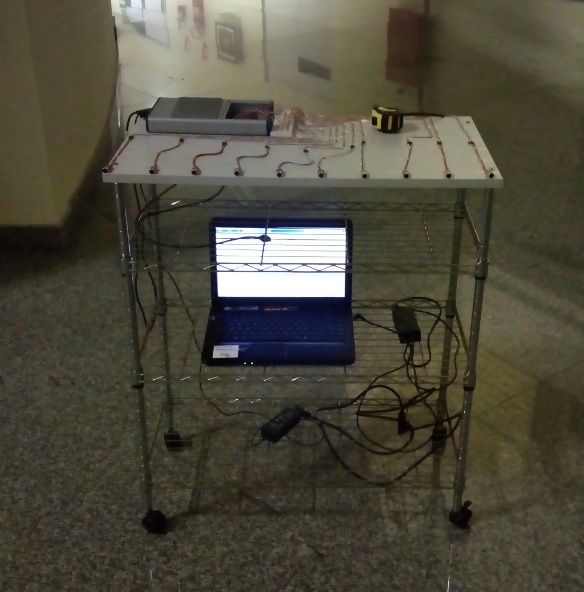
\includegraphics{img8.png}}
\caption{Mesa montada para aquisição.}\label{fig:mesa_pronta}
\end{figure}

Os alunos sempre auxiliam nas medições, e atualmente realizam medições sozinhos. A fonte é uma caixa de som da JBL, de dois modelos, com potência de 4W cada lado. Mostrado nas Figuras \ref{fig:jbl1} e \ref{fig:jbl2}.  

\begin{figure}
\centering
\scalebox{0.5}{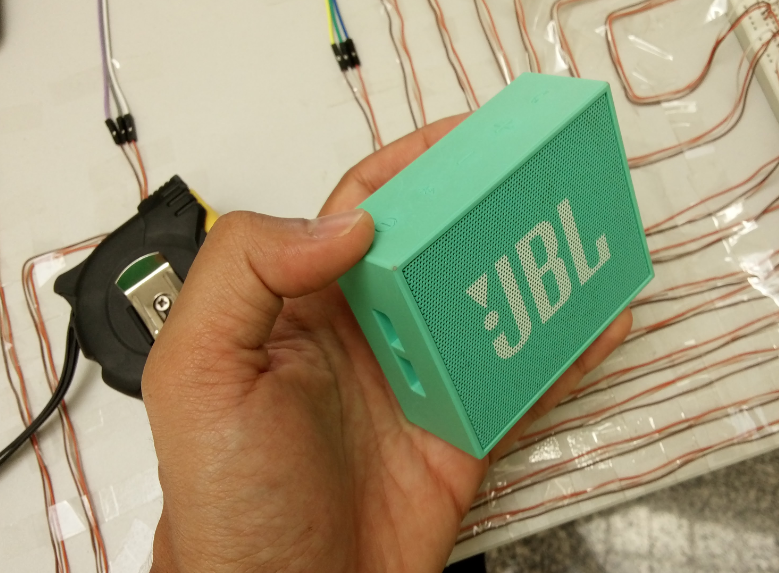
\includegraphics{img10.png}}
\caption{Caixinha JBL 1.}\label{fig:jbl1}
\end{figure}

\begin{figure}
\centering
\scalebox{0.5}{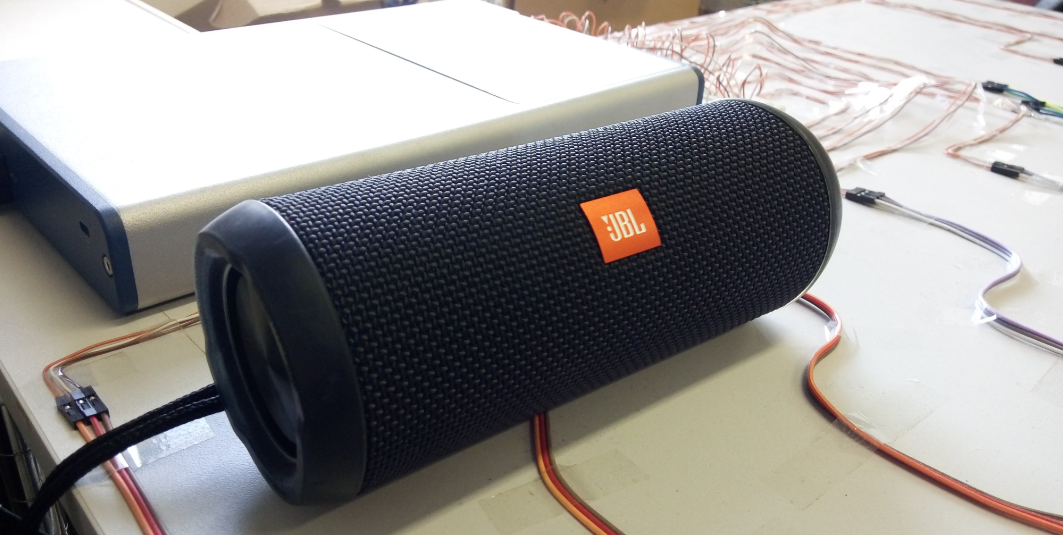
\includegraphics{img11.png}}
\caption{Caixinha JBL 2.}\label{fig:jbl2}
\end{figure}

As aquisições seguem os seguintes passos:

\begin{enumerate}
\item É feito a marcação no chão das posições para ângulos definidos de 0º até 60º com o passo de 5º. A começar pela linha do eixo dos microfones;
\item Inicialização do NI-6361, do notebook e da fonte;
\item Realiza uma primeira aquisição em silêncio;
\item Posiciona a caixa de som nas posições dos ângulos corretas na altura da mesa;
\item Conecta via bluetooth um smartphone com a caixa de som JBL e emite um tom em 1kHz;
\item Realiza aquisições de cerca de 400.000 amostras em cada ângulo. Mostrado na Figura \ref{fig:medicao}.
\end{enumerate}

\begin{figure}
\centering
\scalebox{0.4}{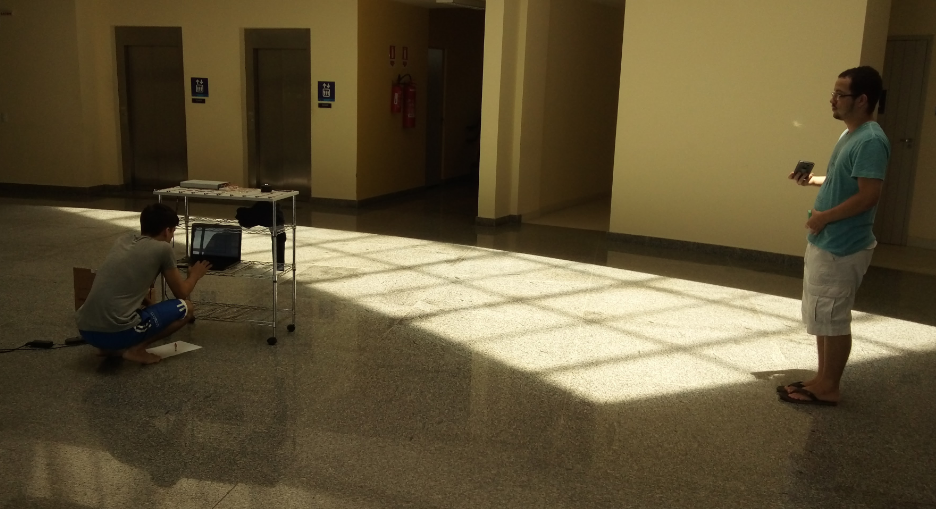
\includegraphics{img9.png}}
\caption{Medição.}\label{fig:medicao}
\end{figure}

\subsection{Medições}

As medições são realizadas pelo período da noite, com menos ruído ambiente, no prédio do CTEC, na UFRN. A distância entre a fonte e o primeiro microfone é especificada na medição, e salva no nome do arquivo medido, conforme a Figura \ref{fig:medicao_fonte}.

\begin{figure}
\centering
\scalebox{0.6}{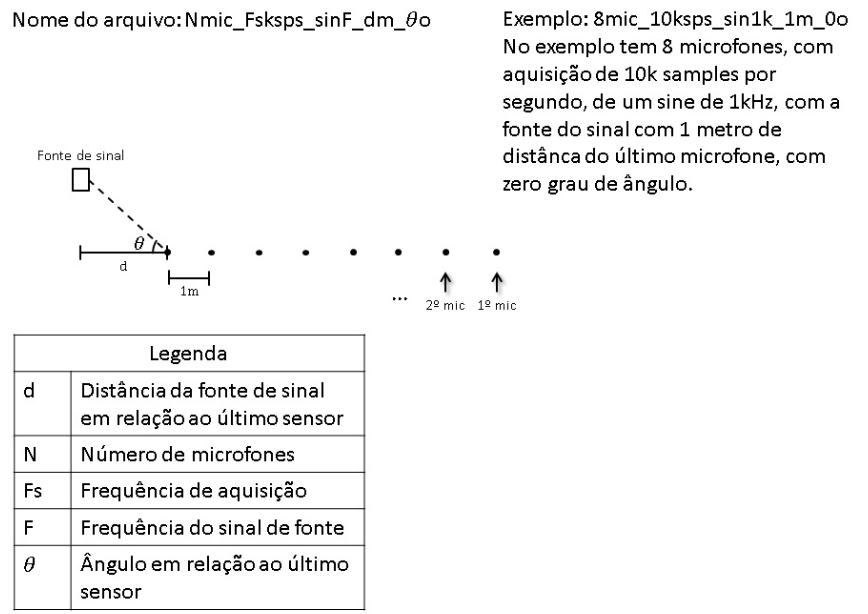
\includegraphics{img12.png}}
\caption{Esquema de medição.}\label{fig:medicao_fonte}
\end{figure}

No nome do arquivo está especificado a distância, o ângulo conhecido, o número de microfones, e a frequência do tom medido. Além do nome do arquivo, é gravado junto um arquivo .txt com detalhes da medição, como data e hora, as pessoas presentes, se houve algum ruído incomum no ambiente, etc.

Atualmente temos medições com distâncias entre 1 a 8 metros entre a fonte e os microfones. Com ângulos de 0 a 60 graus, frequências de tom de 1kHz, com 8 e 10 microfones.

\subsection{Dificuldades}

1. Falta de um computador com RTOS para aquisição de maior quantidade de amostras.

2. Calibragem dos microfones.

3. Precisão nas medidas de ângulo e distância entre fonte e receptores.

4. Falta de estimativa de SNR.

5. Desconhecimento do modelo de canal acústico.

6. Baixa qualidade dos microfones.

%----------------------------------------
\section{Resultados e Conclusões}

Os resultados do ângulo de chegada se encontram nas pastas de resultados dos respectivos algoritmos no Dropbox.

\pagebreak

%----------------------------------------
\section{Referências}

NI-6361 http://www.ni.com/pdf/manuals/374650c.pdf



%----------------------------------------
%\bibliographystyle{abbrvnat}
%\bibliography{relatorio}

\end{document}
